\documentclass[10pt,a4paper,titlepage,oneside]{article}
\usepackage{LabProtocol}
\usepackage{tikz}
\usepackage{enumitem}
\usepackage{hyperref} 

\usepackage{wrapfig}
\usepackage{multirow} 
\usepackage{tabularx}
\usepackage[naustrian]{babel}
\usepackage{float}
\usepackage{todonotes}
\usepackage{fontawesome}
\usepackage{subfig}

\usepackage[utf8]{inputenc}

\renewcommand{\arraystretch}{1.5}

\usetikzlibrary{arrows,automata} 

\exercise{}

% enter your data here
\authors{
	Daniel Zainzinger, Matr. Nr. 11777778 \\Noah Bruns, Matr. Nr. 01630029\par
	{\small e11777778@student.tuwien.ac.at\\ e01630029@student.tuwien.ac.at} \par
}


\begin{document} 

\maketitle  
 
\tableofcontents
\newpage  
\section{Einleitung}
Für das Programmieren mit mehreren Prozessoren ist es oft erforderlich, eine gemeinsame Datenstruktur zu verwenden. 
Eine Möglichkeit ist das List based Set. Dabei handelt es sich um eine Liste, bei welcher jedes Element einen Key besitzt.
Dieser Key ist eindeutig und die gesamte Liste ist anhand dieses Keys sortiert. 
Um das Testen und Benchmarken der Datenstrukturen einfach zu halten, werden nur positive Integer Werte in die Datenstruktur eingefügt (siehe \ref{bench:aufbau}). 
Es gibt mehrere Optionen für die Implementatierung einer solchen Liste. In Folgendem Kapitel werden 5 verschiedene Implementirungen vergestellt die verschidenene Techniken verwenden um die Synchronisierung und den sicheren Zugriff der gemeinsamen Datenstruktur zu gewährleisten. Eine Anleitung zum kompilieren und ausführen kann
aus dem ``README.TXT'' entnommen werden.

\begin{figure}[H]
	\centering 
	\begin{tikzpicture}
		\node[draw,circle,minimum size=1cm,inner sep=0pt] at (0,0) {$- \infty$};
		\draw[->] (0.5,0) -- (1.5,0);
		\node[draw,circle,minimum size=1cm,inner sep=0pt] at (2,0) {$3$};
		\draw[->] (2.5,0) -- (3.5,0);
		\node[draw,circle,minimum size=1cm,inner sep=0pt] at (4,0) {$5$};
		\draw[->] (4.5,0) -- (5.5,0);
		\node[draw,circle,minimum size=1cm,inner sep=0pt] at (6,0) {$8$};
		\draw[->] (6.5,0) -- (7.5,0);
		\node[draw,circle,minimum size=1cm,inner sep=0pt] at (8,0) {$10$};
		\draw[->] (8.5,0) -- (9.5,0);
		\node[draw,circle,minimum size=1cm,inner sep=0pt] at (10,0) {$\infty$};
	\end{tikzpicture}
	\caption{Aufbau der Liste}
	\label{tik:list}
\end{figure}

In der Abbildung \ref{tik:list} wird dargestellt wie eine solche Liste aussieht. Am Anfang und am Ende befinden sich 2 Nodes $-\infty$ und $\infty$ die den 
Anfang und das Ende der Liste markieren. Dazwischen befinden sich in sortierter Reihenfolge die eingefügten Keys.

Jede der Implementierungen enthält 3 Methoden die mit denen die Liste bearbeitet werden kann:

\begin{table}[H]
    \begin{tabularx}{\textwidth}{lX}
        \textit{add} & Fügt ein Elemet in die Liste ein. Falls dieses schon enthalten ist gibt die Methode \textit{false} zurück sonst \textit{true}. \\
        \textit{contains} & Wenn das Element in der Liste gefunden wurde gibt diese Methode \textit{true} oder sonst \textit{false} zurück. \\
        \textit{remove} & Diese Methode entfernt einen Key aus der Liste und gibt \textit{true} zurück. Falls der Key nicht in der Liste vorhanden ist wird \textit{false} zurückgegeben. \\
    \end{tabularx}
\end{table}


\section{Implementierung}
\label{sec:implementation}
\subsection{List-based set with coarse-grained locks}

Bei dieser Implementierung wir vor jedem Methodenaufruf die gesamte Liste gesperrt. Dadurch kann aber die Parallelisierung 
nicht ausgenutzt werden, da zu einem Zeitpunkt maximal ein Prozess auf die Liste zugreifen kann. Diese Implementierung ist 
daher sehr ähnlich zu einer sequentiellen Implementierung.

\begin{figure}[H]
	\centering
    \begin{tikzpicture}
        \draw (-0.5,1) -- (10.5,1) node [midway, above, sloped] {\faLock};
		\node[draw,circle,minimum size=1cm,inner sep=0pt] at (0,0) {$- \infty$};
		\draw[->] (0.5,0) -- (1.5,0);
		\node[draw,circle,minimum size=1cm,inner sep=0pt] at (2,0) {$3$};
		\draw[->] (2.5,0) -- (3.5,0);
		\node[draw,circle,minimum size=1cm,inner sep=0pt] at (4,0) {$5$};
		\draw[->] (4.5,0) -- (5.5,0);
		\node[draw,circle,minimum size=1cm,inner sep=0pt] at (6,0) {$8$};
		\draw[->] (6.5,0) -- (7.5,0);
		\node[draw,circle,minimum size=1cm,inner sep=0pt] at (8,0) {$10$};
		\draw[->] (8.5,0) -- (9.5,0);
		\node[draw,circle,minimum size=1cm,inner sep=0pt] at (10,0) {$\infty$};
	\end{tikzpicture}
	\caption{coarse-grained locks}
	\label{tik:coarse-grained}
\end{figure}

\begin{table}[H]
    \begin{tabularx}{\textwidth}{lX}
        \textit{add} & Nachdem die Liste gesperrt wurde, wird sie durchlaufen bis zu dem Punkt, an dem der Key des betrachteten Nodes größer ist als der einzufügende ist. Vor diesen wird der neue Node eingefügt. \\
        \textit{contains} & Die Liste wird gesperrt und dann durchlaufen. Wenn dabei der gesuchten Wert gefunden wird, wird \textit{true}, ansonsten \textit{false} zurückgegeben.\\
        \textit{remove} & Nachdem die gesamte Liste gesperrt wurde wird das Element in der Liste gesucht und entfernt.\\
    \end{tabularx}
\end{table}

\subsection{List-based set with fine-grained locks}

Im Unterschied zu den \textit{coarse-grained locks} wird bei dieser Implementierung immer nur der derzeitige Node gesprerrt. 
Beim Iterieren der Liste wird während dem Übergang zum nächsten Node die derzeitige und der darauffolgende Node gesperrt. 
Ein Node kann zu einem Zeitpunkt nur von einem Prozess gesperrt sein. Der Vorteil gegenüber den coarse-grained locks besteht darin, 
dass nun wirkliche Parallelisierung möglich ist und verschiedene Threads an unterschiedlichen Punkten an der Liste arbeiten können. 
Es hat jedoch den Nachteil, dass die Iterationsgeschwiendigkeit durch den langsamsten Thread definiert wird, da ein 
Thread in der Liste nicht ``Überholt'' werden kann.

\begin{figure}[H]
	\centering
    \begin{tikzpicture}
        \draw (3.5,1) -- (4.5,1) node [midway, above, sloped] {\faLock};
        \draw (5.5,1) -- (6.5,1) node [midway, above, sloped] {\faLock};
		\node[draw,circle,minimum size=1cm,inner sep=0pt] at (0,0) {$- \infty$};
		\draw[->] (0.5,0) -- (1.5,0);
		\node[draw,circle,minimum size=1cm,inner sep=0pt] at (2,0) {$3$};
		\draw[->] (2.5,0) -- (3.5,0);
		\node[draw,circle,minimum size=1cm,inner sep=0pt] at (4,0) {$5$};
		\draw[->] (4.5,0) -- (5.5,0);
		\node[draw,circle,minimum size=1cm,inner sep=0pt] at (6,0) {$8$};
		\draw[->] (6.5,0) -- (7.5,0);
		\node[draw,circle,minimum size=1cm,inner sep=0pt] at (8,0) {$10$};
		\draw[->] (8.5,0) -- (9.5,0);
		\node[draw,circle,minimum size=1cm,inner sep=0pt] at (10,0) {$\infty$};
	\end{tikzpicture}
	\caption{fine-grained locks}
	\label{tik:fine-grained}
\end{figure}

\begin{figure}[H]
	\centering
    \begin{tikzpicture}
        \draw (3.5,1) -- (4.5,1) node [midway, above, sloped] {\faLock};
        \draw (5.5,-1) -- (6.5,-1) node [midway, above, sloped] {\faLock};
		\node[draw,circle,minimum size=1cm,inner sep=0pt] at (0,0) {$- \infty$};
		\draw[->] (0.5,0) -- (1.5,0);
		\node[draw,circle,minimum size=1cm,inner sep=0pt] at (2,0) {$3$};
		\draw[->] (2.5,0) -- (3.5,0);
		\node[draw,circle,minimum size=1cm,inner sep=0pt] at (4,0) {$5$};
        \draw[->] (4.5,0) -- (7.5,0);
        \draw[line width=0.5mm, red] (5.5,-1.5) -- (6.5,-2.5);
        \node[draw,circle,minimum size=1cm,inner sep=0pt] (A) at (6,-2) {$8$};
        \node[draw,circle,minimum size=1cm,inner sep=0pt] (B) at (8,0) {$10$};
        \draw[->] (A) -- (B);
		\draw[->] (8.5,0) -- (9.5,0);
		\node[draw,circle,minimum size=1cm,inner sep=0pt] at (10,0) {$\infty$};
	\end{tikzpicture}
	\caption{fine-grained locks remove}
	\label{tik:fine-grained-remove}
\end{figure}

\begin{table}[H]
    \begin{tabularx}{\textwidth}{lX}
		\textit{add} & Die Liste wird mit locks iteriert, bis der Punkt an dem der Node eingefügt werden soll erreich ist. Beim erreichen diese Punktes ist
		 sowohl der Vorgänger als auch der Nachfolger bereits gesperrt. Dadurch kann der neue Node sicher eingefügt werden.\\
		\textit{contains} & Die Liste wird analog zur coarse-grained locks iteriert, dabei aber immer der derzeitige Node bzw. beim Übergang Vorgänger und Nachfolger gesperrt. 
		Wenn der entsprechende Node gefunden wurde, wird \textit{true} sonst \textit{false} zurückgegeben. \\
		\textit{remove} & Die Liste wird wie bei \textit{contains} iteriert. Sobald der zu entfernende Node gefunden wurde, wird der Zeiger des vorgänger Nodes
		auf den darauffolgenden verwiesen und somit der zu entfernende Node übersprungen. Da der löschende Thread durch den lock exklusiven Zugriff auf den Node hat,
		kann dieser auch physikalisch vom Speicher entfernt werden. 
		Siehe Abbildung \ref{tik:fine-grained-remove}\\
    \end{tabularx}
\end{table}


\subsection{List-based set with optimistic synchronization}

In dieser Implementierung wird beim Suchen eines Elementes zuerst kein Node gesperrt, sondern einfach nur eine Iteration durchgeführt. 
Sobald der gesuchte gefunden wurde, wird dieser gesperrt. Anschließend muss sichergestellt werden, dass dieser Node noch immer erreichbar ist 
und nicht von einem anderen Thread bereits gelöscht wurde. Dies erfordert jedoch eine zweite Iteration der Liste. Ist der Node nicht mehr erreichbar, 
wird der Algorithmus von vorne gestartet. Dies hat den Vorteil, dass beim Suchen eines Keys in der Liste keine Sperrungen benötigt werden. 
Erst wenn das Element gefunden wurde, wird es gesperrt. Jedoch sind dadurch zwei Iterationen notwendig.

\begin{table}[H]
    \begin{tabularx}{\textwidth}{lX}
		\textit{add} & Beim Hinzufügen wird die Liste durchlaufen ohne Nodes zu sperren bis der entsprechende Punkt zum Einfügen gefunden wurde. 
		Die vorgänger und nachfolger Nodes werden gesperrt und mittels erneutem durchlaufen der Liste wird sichergestellt, dass diese Nodes immernoch Teil der 
		Liste sind. Falls dies scheitert wird der Prozess von vorne gestartet. Sind jedoch die gesperrten Nodes immernoch erreichbar, so wir der neue Key 
		zwischen den gesperrten eingefügt und die Sperre wird aufgehoben.\\
		\textit{contains} & Hier wird ebenfalls die Liste ohne Sperrungen durchsucht und nach Erfolgreichen Sperren plus der Validierung der Erreichbarkeit 
		der Nodes wird das Ergebnis zurückgegeben.\\
		\textit{remove} & Gleich wie bei den anderen Methoden wird der Key gesucht, gesperrt und validiert. Danach wird das Element aus der Liste entfernt und 
		alle Sperrungen werden aufgehoben. Da für das Iterieren keine Sperrungen erforderlich sind, kann nicht sichergestellt werden, dass der ausgelinkte
		Node nicht von einem anderen Thread gerade gelesen wird. Dadurch kann der Node nicht vom Speicher gelöscht werden.\\
    \end{tabularx}
\end{table}

Bei dieser Implementierung wurde auf Memory Managemen verzichtet, dadurch wird Speicher geleakt.
Eine Lösung dieses Problems wird in Kapitel \ref{sec:mem} gezeigt.

\subsection{List-based set with lazy synchronization}

Lazy Synchronization verwendet eine Markierung auf den Nodes welche bekannt gibt, ob dieser Node bereits logisch gelöscht wurde. 
Bei einem Lösch-Vorgang wird der zu löschenden Node diese Markierung gesetzt. Dadurch wird dieser Node bei anderen Methoden, 
wie zum Beispiel \textit{contain()} oder \textit{add()}, ignoriert. Dies hat den Vorteil, 
dass für den Aufruf von der \textit{contains()} Methode keine Sperrungen und keine Validierung erforderlich ist.
Dies bringt eine Performancesteigerung, da in der Regel mit \textit{contain()} die meisten Zugriffe auf die Datenstruktur erfolgen. 


\begin{figure}[H]
	\centering
    \begin{tikzpicture}
		\node[draw,circle,minimum size=1cm,inner sep=0pt] at (0,0) {$- \infty$};
		\draw[->] (0.5,0) -- (1.5,0);
		\node[draw,circle,minimum size=1cm,inner sep=0pt] at (2,0) {$3$};
		\draw[->] (2.5,0) -- (3.5,0);
		\node[draw,circle,minimum size=1cm,inner sep=0pt] at (4,0) {$5$};
        \draw[->] (4.5,0) -- (7.5,0);
        \node[draw,circle,minimum size=1cm,inner sep=0pt] (A) at (6,-2) {$8$};
        \node[draw,circle,minimum size=0.8cm,inner sep=0pt, red] at (6,-2) {};
        \node[draw,circle,minimum size=1cm,inner sep=0pt] (B) at (8,0) {$10$};
        \draw[->] (A) -- (B);
		\draw[->] (8.5,0) -- (9.5,0);
		\node[draw,circle,minimum size=1cm,inner sep=0pt] at (10,0) {$\infty$};
	\end{tikzpicture}
	\caption{fine-grained locks remove}
	\label{tik:fine-grained-remove}
\end{figure}

\begin{table}[H]
    \begin{tabularx}{\textwidth}{lX}
        \textit{add} & Gleich wie bei den optimistic synchronization\\
		\textit{contains} & Die Liste wird durchlaufen und bei einem erfolgreichem Fund wird sichergestellt, dass dieses Element noch nicht markiert wurde.
		Durch diese Markierung ist keine Validierung erforderlich. \\
		\textit{remove} & Der Key wird gesucht und mitsamt seinem Vorgänger gesperrt. Danach wird Validiert, ob dieses Element immernoch erreichbar ist. 
		Wenn dies der Fall ist wird das Element markiert und einseitig aus der Liste entfernt. Das bedeutet, dass dieser Node weiterhin auf den Nachfolger 
		zeigt, aber nicht mehr vom Kopf erreicht werden kann. Dies ist in Abbildung \ref{tik:fine-grained-remove} verdeutlicht. Dadurch kann wie bei
		optimistic synchronization der Node nicht vom Speicher entfernt werden.\\
    \end{tabularx}
\end{table}

Bei dieser Implementierung wurde auf Memory Managemen verzichtet, dadurch wird Speicher geleakt.
Eine Lösung dieses Problems wird in Kapitel \ref{sec:mem} gezeigt.



\subsection{Lock-free list-based set}

Das Ziel dieser Implementierung ist es eine sperrungsfreie Liste zu erstellen. Dazu wird ähnlich wie bei der \textit{lazy synchronization} eine Markierung verwendet. 
Diese Markierung wird aber in den next-Pointer des Nodes integriert, damit beide \textit{atomic} gelesen und geschrieben werden können. 
Um dies zu ermöglichen kann einfach ein Bit des Pointers genommen werden. Da bei einem 64-Bit Computer nicht alle Bits für die Adressierung 
des Speichers verwendet werden, kann das höchste Bit als Markierung umfunktioniert werden.

\begin{table}[H]
    \begin{tabularx}{\textwidth}{lX}
		\textit{add} & Bei add wird zuerst der Punkt zum Einfügen gesucht und dann wird ein neuer Node erzeugt, welcher auf den nachfolger Node zeigt. 
		Danach wird mittels \textit{compare\_exchange} der Vorgänger auf den neuen Node verwiesen und somit der neue Node in die Liste atomar eingefügt. 
		Scheitert \textit{compare\_exchange}, weil der next-Pointer vom Vorgänger von einem anderen Thread verändert wurde, wird der Prozess von Neuem gestartet. \\
        \textit{contains} & Gleich wie bei \textit{lazy synchronization} \\
		\textit{remove} & Bei remove wird der zu entfernende Node zuerst gesucht und dann im next-Pointer markiert. 
		Danach wird wieder mittels \textit{compare\_exchange} versucht 
		die Node noch aus der Liste zu entfernen indem in der Vorgänger Node der next-Pointer auf den Nachfolger gelegt wird. Falls dies jedoch scheitert werde 
		keine werteren Versuche zum Entfernen des Nodes aus der Liste vorgenommen. Die \textit{find()} Funktion, welche von \textit{add()}, \textit{contain()} und 
		\textit{remove()} verwendet wird, erkennt beim Iterieren markierte Nodes und versucht erneut diese zu entfernen. \\
    \end{tabularx}
\end{table}

\subsubsection{Verbesserungen}
\label{subsec:impr}
In der \textit{find} Funktion wird für das Auslinken eines Nodes wird ein Compare and Swap(CAS) verwendet. Falls dies fehlschlägt, 
weil z.b. der Node zum beispiel bereits ausgelinkt wurde,
wird wieder beim Listenkopf begonnen. Um dieses Verhalten zu verbessern, wurde in \textit{Lock\_free\_impr.cpp} folgendes implementiert:\\
Es wird immer der alte \textit{predecessor} gespeichert. Sollte CAS fehlschlagen, wird überprüft ob der alte \textit{predecessor}
zum auslinken markiert wurde. Ist dies der Fall, werden \textit{predecessor, current} und \textit{successor} auf den jeweiligen Vorgänger
gesetzt und an dieser Stelle weitergemacht. 
\section{Memmory Managment}\label{sec:mem}
Bei \textit{List-based set with optimistic synchronization}, \textit{List-based set with lazy synchronization} und \textit{Lock-free list-based set}
gibt es ein Problem mit den Memmory Managment. Bei diesen Datenstrukturen ist das lesen eines Nodes auch ohne einen Lock möglich. 
Dadurch kann von einen Thread nicht sichergestellt werden, dass nach dem auslinken eines Nodes dieser nicht noch von einen anderen Thread gelesen wird.
\\ 
\textbf{Beispiel:}
\\ Angenommen Thread A liest einen Node und legt sich schlafen. Thread B will diesen Thread löschen. Dazu linkt er den Node aus der Datenstruktur aus
. Anschließend wird dieser von Thread B gelöscht. Wenn nun Thread A wieder aufwacht, und auf den Node zugreiffein will, ist der Speicher bereits freigegeben
und es tritt ein Segfault auf. 

\subsection{Markierung beim Lesen}
Als erster Ansatz wurde versucht, mithilfe eines Counters einen Node zu markieren, dass dieser gerade gelesen wird. Dieser Ansatz ist jedoch nicht 
Zielführend und ist nur zum verdeutlichen der Schwierigkeit dieses Problems erwähnt. \\
Bevor ein Thread einen Node liest, erhöht er einen Counter in diesen Node. Nachdem ein Node verlassen wurde, wird dieser Counter wieder verringert.
Ein Thread, der diesen Node löschen will, darf dies erst tun, sobald der Node ausgelinkt und der Counter den Wert 0 hat. \\
Damit ein Thread den nächsten Node markieren kann, muss er zuerst den ``next'' Pointer aus den aktuellen Node auslesen und dann den Counter erhöhen (next$\rightarrow$counter++).
Es ist jedoch nicht möglich, das Auslesen des next Pointers und das erhöhen des Counters atomar auszuführen. Auch ein ``compare and swap'' ist hierbei nicht hilfreich,
da das vergleichen mit einen freigegebenen Speicherbereich zu einen Segmentation Fault führt. 


\subsection{Delete Queue mit Zeitstempel}
Um zu vermeiden, dass ein Node gelöscht wird, während er von einen anderen Thread noch gelesen wird, muss sichergestellt werden, dass dieser ``frei'' ist. 
Dazu wurden Zeitstempel eingeführt. Jeder Thread besitzt einen globalen Integer, wo sein Zeitstempel gespeichert wird. Sobald eine Operation
wie Beispielsweise ``add'' abgeschlossen ist, wird dieser Zeitstempel erhöht.  Will nun ein Thread einen Node löschen, wird dieser zuerst ausgelinkt. 
Anschließend werden alle Zeitstempel ausgelesen und gemeinsam mit einen Pointer auf den zu löschenden Node in einer Queue hinzugefügt. Diese 
Queue wird lokal im Thread gespeichert und wurde als C++ Vektor realisiert. Nach den Abschluss einer Operation wie Beispielsweise ``add'', wird 
die Queue mit zu löschenden Kandidaten durchlaufen. Für jeden Node werden nun die gespeicherten Zeitstempel mit den aktuellen Zeitstempel verglichen. 
Wenn sich alle Zeitstempel eines Nodes von den aktuellen Zeitstempel unterscheiden, ist sichergestellt, dass dieser Node von keinen Thread mehr gelesen wird. 
Nun kann der Speicher des Nodes wieder Freigegeben werden und aus der Queue entfernt werden. 
\\Bevor ein Thread geschlossen wird, muss sichergestellt werden
dass die Queue gelehrt wird und somit der Speicher aller Kandidaten gelöscht wird. Da hierbei die Zeitstempel nicht mehr überprüft werden,
kann die Liste nach dem Schließen eines Threads nicht mehr verwendet werden. 
\section{Benchmark}
Beim Ausführen von ./main wird ein Benchmark Test durchgeführt. Dieser gibt die jeweils benötigte Zeit aus und erstellt ein .csv für jede Datenstruktur
in den ``result'' folder. 

\subsection{Aufbau}
\label{bench:aufbau}
Es werden zwei files für einen Test benötigt: pre[0-9]+.csv und main[0-9]+.csv. Mithilfe der Einträge im pre-file wird die
Datenstruktur befüllt. Sobald dies abgeschlossen ist, werden alle negativen Werte im main-file aus der Datenstruktur gelöscht 
und alle positiven Einträge hinzugefügt. Somit sind in der Liste nur positive Werte zulässig. Die implementierten Datenstrukturen
würden grundsätzlich aber auch mit negativen Werten und anderen Datentypen funktionieren. Um jedoch einen einfachen 
Benchmark zu realisieren sind nur Einträge zwischen 1 und 2.147.483.646 möglich. 
Nach jeder Entfernung und Hinzufügung eines Wertes wird mithilfe von \textit{contain()} überprüft, ob das Element hinzugefügt bzw.
entfernt wurde. 
Als dritter und letzter Schritt wird mithilfe von \textit{contain()} überprüft, ob sich alle positiven Werte aus dem main-File 
in der Datenstruktur befinden und ob alle negativen Werte aus der Datenstruktur entfernt wurden. 
\\
pre[0-9]+.csv und main[0-9]+.csv sind so aufgebaut, dass im main-File alle Werte aus dem pre-file mit negativen Vorzeichen
vorhanden sind und die positiven Werte nicht im pre-File vorkommen. Desweiteren werden alle Einträge in den beiden Files
zufällig permutiert. 

\subsection{Testcases erstellen}
Die Testcases werden mithilfe eines Python Skriptes erstellt. Dabei ist die Größe der Testcases mithilfe der Konstanten
RAW\_BASE und COOLUMS\_BASE einzustellen. Mit FILE\_AMOUNT kann eingestellt werden, wie viele Testcases erstellt werden.
Dabei werden bei jeder Interation RAW\_BASE und COOLLUM\_BASE mit 2 hoch der aktuellen Iteration-Variable multipliziert. 


\subsection{Interpretation Benchmark Werte}
Die Dauer jedes einzelnen Tests und ob der Test erfolgreich war wird in der Kommandozeile ausgegeben. Desweiteren wird
im Ordner \textit{results} für jede Datenstruktur ein CSV File angelegt. Die Beschreibung der einzelnen 
Features kann aus Tabelle \ref{tab:csv} entnommen werden.
\begin{table}[H]
	%\begingroup

	\setstretch{1.2}
	%\renewcommand{\arraystretch}{1.5} % Default value: 1
	\begin{tabular}{ |m{2.5cm}|  m{13cm}| } 

		\hline
	\multicolumn{2}{|l|}{\textbf{Algemeines}}  \\  \hline
	 Cores: & 		Anzahl der verwendeten Cores    \\ \hline
	 TestSizePre& 	Anzahl der Werte, die im ersten Schritt in die Datenstruktur eingefügt wurden\\ \hline
	 TestSizeMain& 	Anzahl der Werte, die im zweiten Schritt hinzugefügt oder entfernt wurden\\ \hline
	 
	 \multicolumn{2}{l}{} \\ \hline
	 \multicolumn{2}{|l|}{\textbf{Ausschließliches einfügen in die Datenstruktur nur \textit{add()}}}    \\ \hline
	 time write& 	Benötigte Zeit, um die Werte aus dem ersten Schritt in die Datenstruktur einzufügen\\ \hline
	 goToStart write& Anzahl der Vorfälle, die ein erneutes Durchsuchen der Datenstruktur vom Beginn an erfordern\\ \hline
	 lostTime write&  Zeit die durch ein erneutes Durchsuchen verloren geht.\\ \hline
	 \multicolumn{2}{l}{} \\ \hline
	 \multicolumn{2}{|l|}{\textbf{Gemischter Zugriff \textit{add(), remove()} und \textit{contain()}}}    \\ \hline
	 time mixed& 	Benötigte Zeit, um die Werte aus dem zweiten Schritt in die Datenstruktur einzufügen 
	 				bzw. zu entfernen und jeweils anschließend zu überprüfen\\ \hline
	 goToStart mixed& Anzahl der Vorfälle, die ein erneutes Durchsuchen der Datenstruktur vom Beginn an erfordern\\ \hline
	 lostTime mixed& Zeit die durch ein erneutes Durchsuchen verloren geht.\\ \hline
	 \multicolumn{2}{l}{} \\ \hline
	 \multicolumn{2}{|l|}{\textbf{Lesender Zugriff nur \textit{contain()}}}    \\ \hline
	 time check& Benötigte Zeit, um zu überprüfen, ob alle Werte aus dem zweiten Schritt hinzugefügt bzw. entfernt wurden \\ \hline
	 goToStart check& Anzahl der Vorfälle, die ein erneutes Durchsuchen der Datenstruktur vom Beginn an erfordern\\ \hline
	 lostTime check& Zeit die durch ein erneutes Durchsuchen verloren geht.\\ \hline
	\end{tabular} 
	\caption{CSV Spalten}
	\label{tab:csv}
	\end{table}

\subsection{Wiederholungen}
Um ein möglichst genaues Ergebnis zu erhalten, müssen die Benchmarks wiederholt werden. Dazu steht in \textit{benchmark.hpp}
die Konstante REPEAT\_TESTS zur Verfügung. In den CSV-Files werden dann die Durchschnittswerte aller Wiederholungen eingetragen. 
\section{Resultate}
Bei den Resultaten handelt es sich um die Datenstrukturen, welche in Kapitel \ref{sec:implementation} beschreiben sind.
Bei Erweiterung ``\_impr'' handelt es sich um eine Verbesserte Version vie in Kapitel \ref{sec:mem} beschrieben.
Bei Datenstrukturen mit der Erweiterung ``\_mem'' ist ein Memorymanagement implementiert (siehe \ref{sec:mem}).
Alle Benchmarks wurden auf den TU Nebula Maschine ausgeführt. Aufgrund der beschrankten Rechenzeit auf dieser Maschine,
wurden die Test nur 10 Mal wiederholt. Die folgenden Abbildungen zeigen jeweils den Mittelwert aller Wiederholungen.

\subsection{Laufzeit mit 64 Cores}

\subsubsection{Schreibvorgang}
\begin{figure}[ht!]
	\centering
	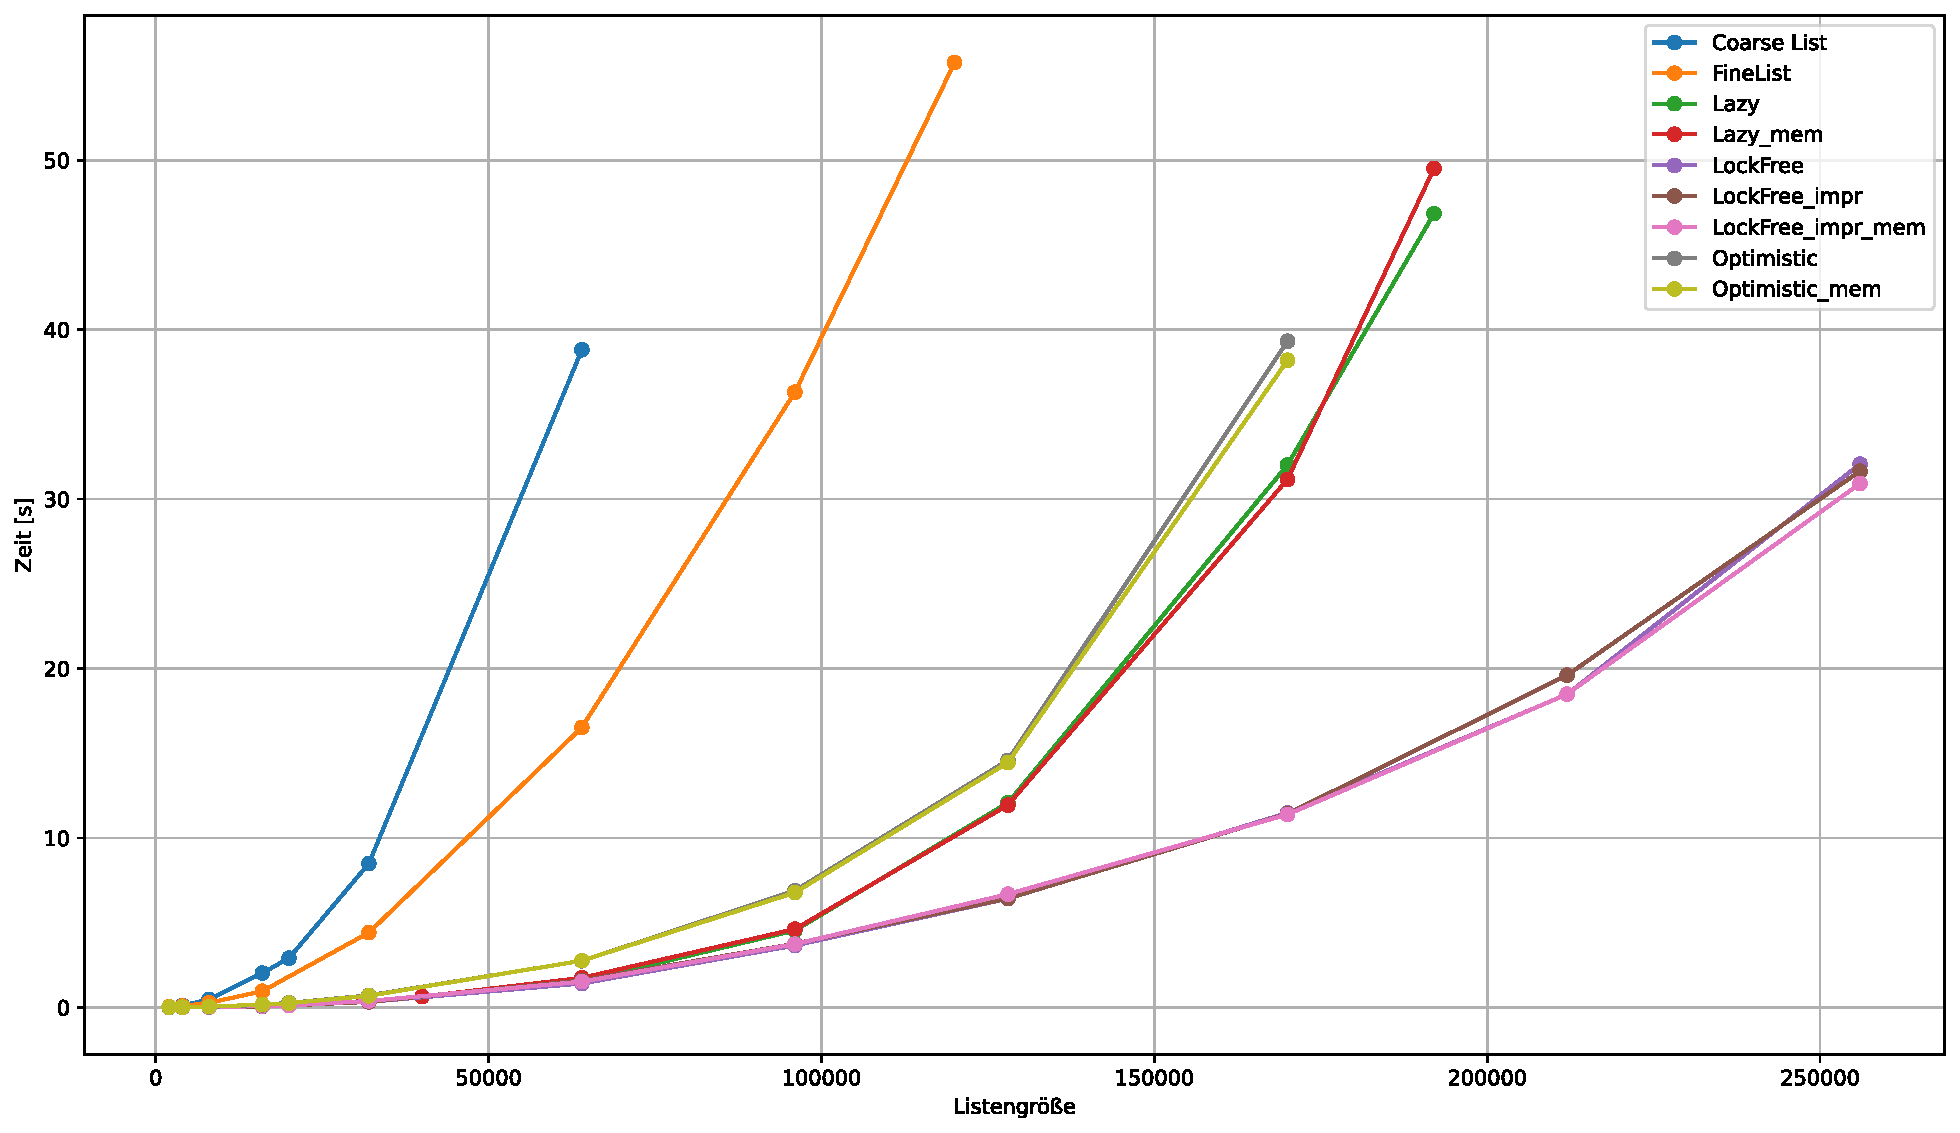
\includegraphics[width=1.0\linewidth]{./plots_pdf/write_time} 
	\caption{Laufzeit des Schreibvorganges}
	\label{fig:write_time} 
\end{figure}
Die Abbildung \ref{fig:write_time} zeigt die benötigte Laufzeit in Sekunden für das Einfügen von Elementen in eine leere Liste.
Dabei ist auf der X-Achse die Anzahl der eingefügten Elemente zu sehen. 
Das \textit{List-based set with coarse-grained locks} ist dabei am Langsamsten, da nur jeweils ein Node gleichzeitig 
Zugriff auf die Liste hat. Die schnellste Datenstruktur ist die \textit{lock-free improved with memorymanagement} Liste.

\subsubsection{Gemischter Zugriff}
\begin{figure}[ht!]
	\centering
	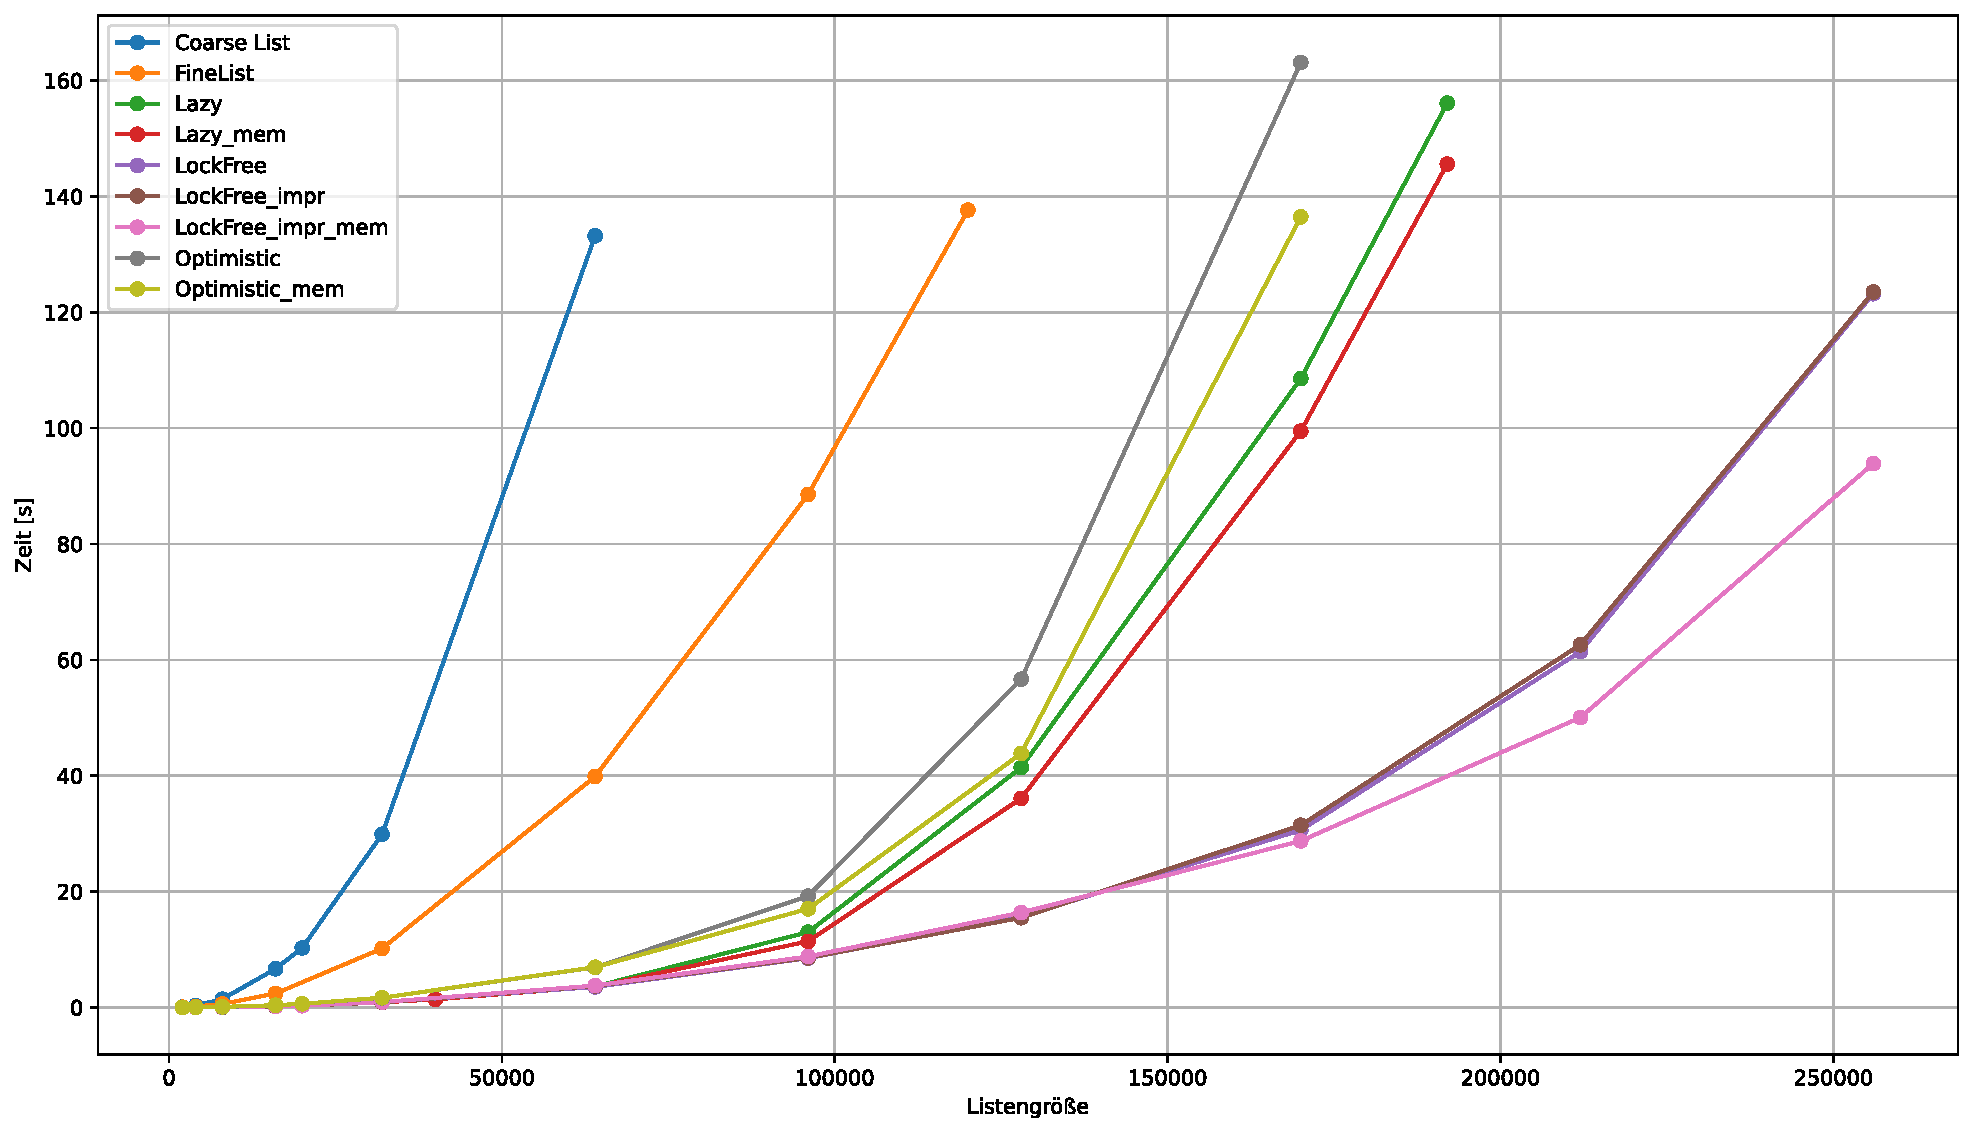
\includegraphics[width=1.0\linewidth]{./plots_pdf/mixed_time} 
	\caption{Laufzeit bei gemischten Zugriff}
	\label{fig:mixed_time} 
\end{figure}
Die Abbildung \ref{fig:write_time} zeigt die benötigte Laufzeit bei gemischten Zugriff. Dabei sind die Zugriffe folgendermaßen aufgeteilt:
 $50\%$ \textit{contain()}, $25\%$ \textit{add()} und $25\%$ \textit{remove()}.
 Dabei ist auf der X-Achse die größe der Liste zu sehen, was auch jeweils der Anzahl der hinzugefügten und entfernten Daten entspricht. 
 Auffallend ist hier, dass Datenstrukturen mit einem implementierten Memorymanagement bei großen Listen schneller sind, obwohl
 das Memorymanagement zusätzlichen aufwand bedeutet. Eine mögliche Begründung liegt darin, dass dem Betriebssystem immer wieder 
 Speicher zurückgegeben wird und somit das auslagern von Daten aus dem Cache minimiert wird.

\subsubsection{Lesender Zugriff}
\begin{figure}[ht!]
	\centering
	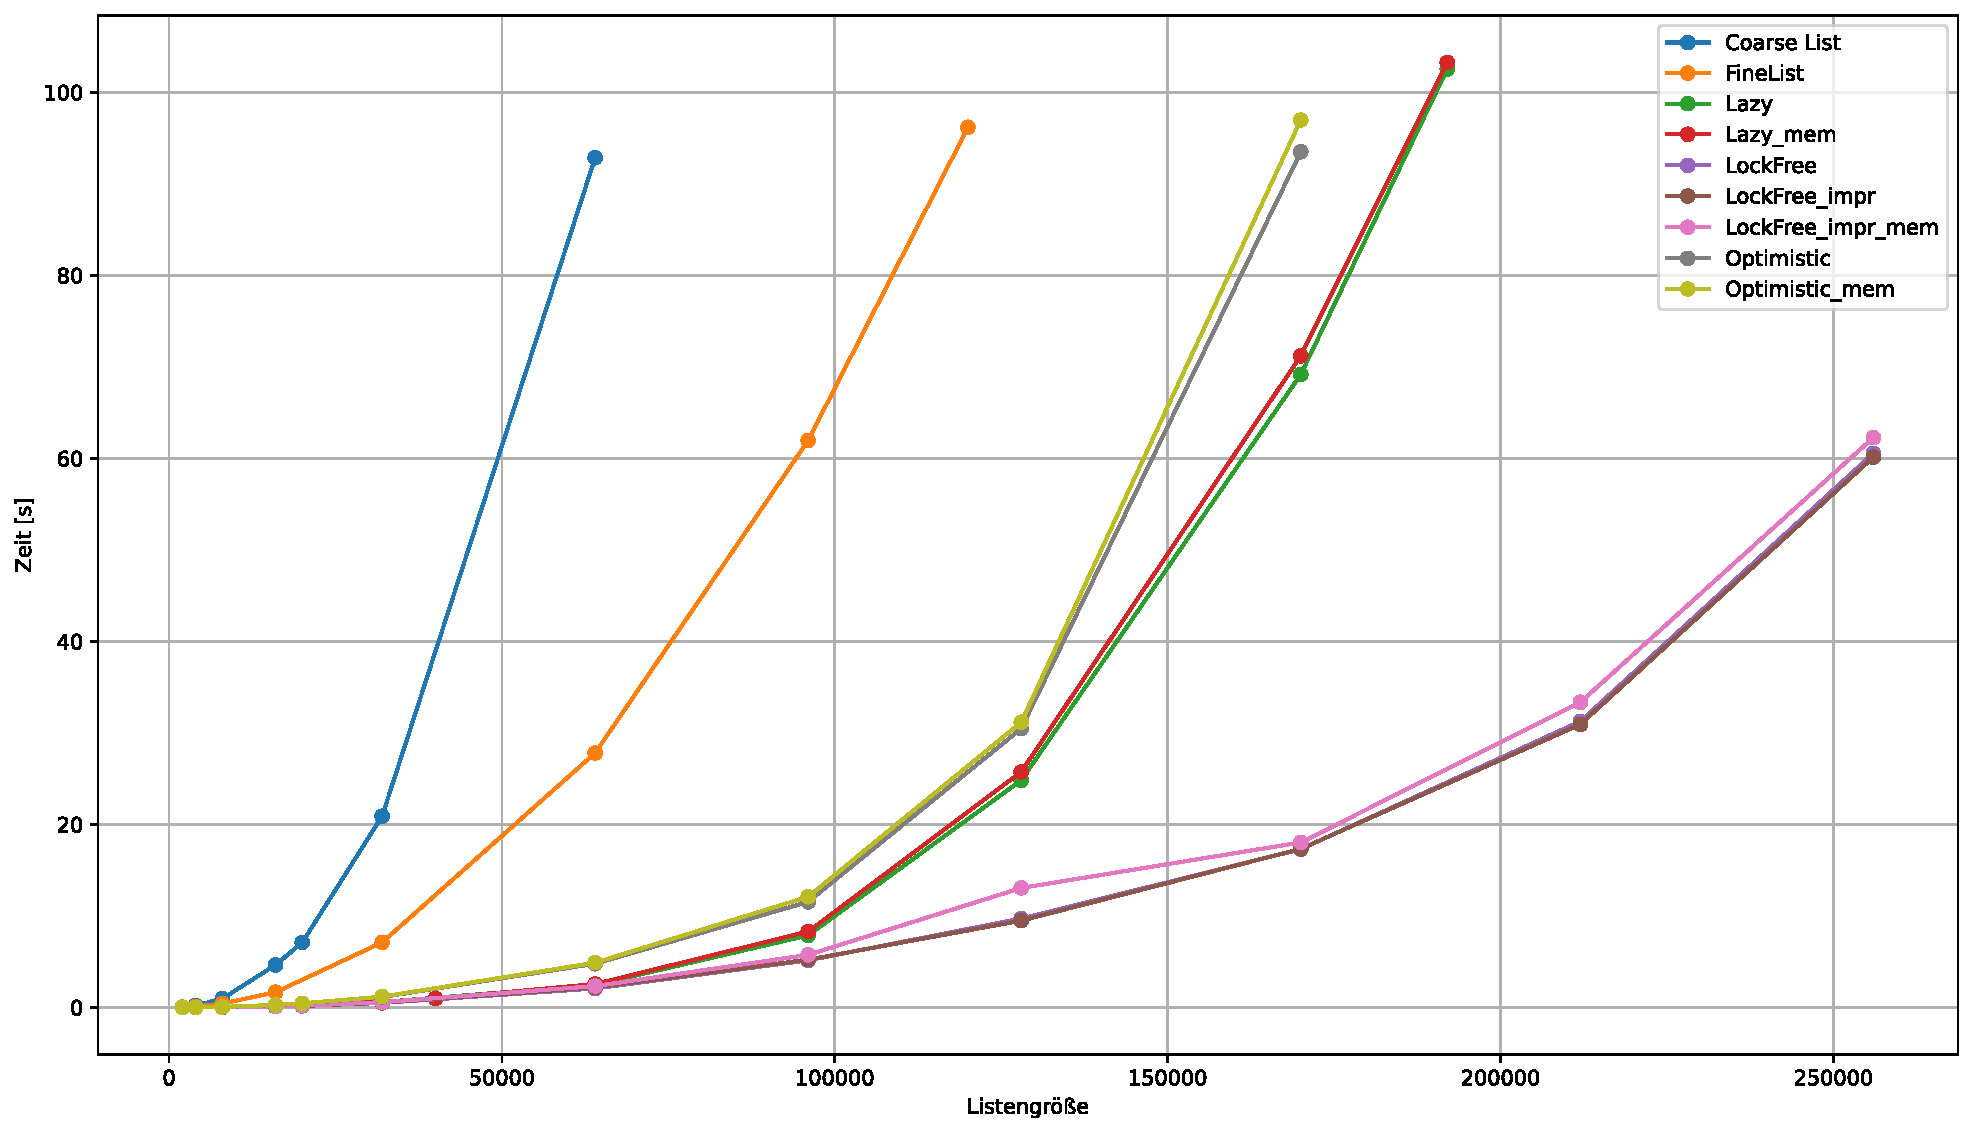
\includegraphics[width=1.0\linewidth]{./plots_pdf/check_time} 
	\caption{Laufzeit für Lesevorgang}
	\label{fig:check_time} 
\end{figure}
Die Abbildung \ref{fig:check_time} zeigt die benötigte Laufzeit, wenn auf die Datenstruktur nur mit \textit{contain()} zugegriffen wird.
Dabei wurden alle Listenelemente abgefragt. Desweiteren wurde die selbe Anzahl an Daten abgefragt, welche sich nicht in der Datenstruktur befinden.
Somit wurden doppelt so viele \textit{contain()} Anfragen ausgeführt, wie Listenelemente vorhanden sind.
Auffallend ist hier, dass beispielsweise die Lazy-Liste bei großen Listen erheblich länger benötigt, als die Lock-free list, obwohl die
\textit{contain()} Funktionen fast identisch sind. Eine mögliche Ursache ist die unterschiedliche größe der Nodes. Die Lazy-Liste beinhaltet
in ihren Nodes zusätzlich eine Variable für Mutex und einen Boolean-Variable zum markieren der gelöschten Nodes. Dieser Größenunterschied könnte für das
Memorymanagement des Betriebssystem einen erhöhten Aufwand beim laden der Nodes beim durchlaufen bedeuten. Dies ist jedoch eine Vermutung
und konnte nicht bestätigt werden.


\subsection{Neustarts von Zugriffen}
Wie bereits in Kapitel \ref{subsec:impr} beschrieben, kann es vorkommen, dass Datenstrukturen aufgrund eines konfliktes mit einem anderen
Thread einen laufenden Task neu beginnen müssen. 
In Abbildung \ref{fig:mixed_lostTime} ist zu sehen, wie oft eine laufende Funktion abgebrochen werden musste und wieder beim Listenkopf beginnen musste. 
In Abbildung \ref{fig:mixed_goToStart} ist ersichtlich, wie viel Zeit für diese Neustarts aufgewendet werden musste. \\
Bei einer Listengröße von 256 000 mit 64 Cores und 512 000 Zugriffen startet die Lock-free Liste 3163 mal neu. Dies bedeutet
einen zusätzlichen Zeitaufwand von 21 Sekunden. Somit spendet jeder Core 0,33 Sekunden mit Neustarts. Bei einer Laufzeit von 123204 Sekunden 
entspricht das 0,00028\% der Laufzeit. Da wie in Abbildung \ref{fig:mixed_lostTime} ersichtlich, steigt die zusätzliche Zeit durch Neustart exponentiell.
Somit wird dies bei noch größeren Listen relevant. Im zuge dieses Projektes wurden jedoch keine größeren Listen getestet. 

\begin{figure}[ht!]
	\centering
	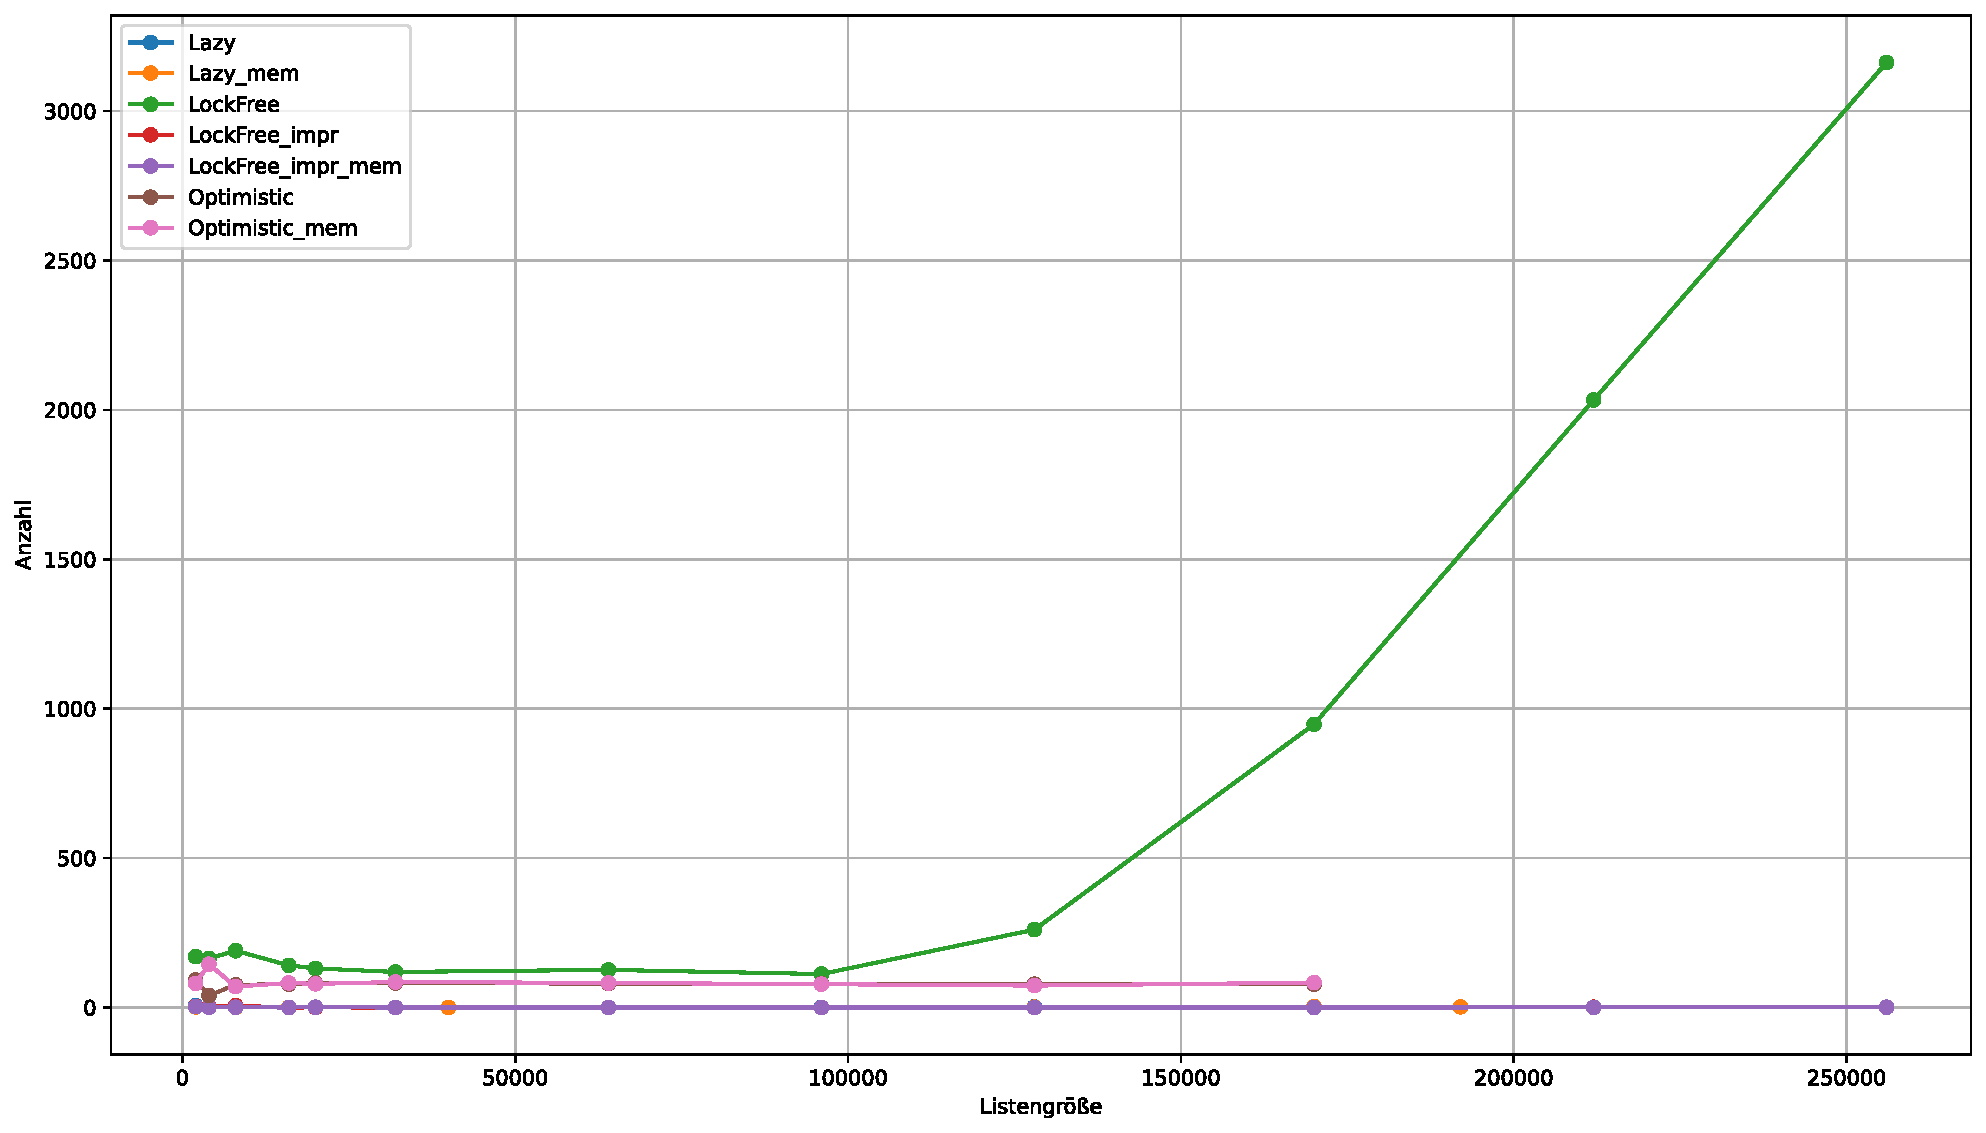
\includegraphics[width=1.0\linewidth]{./plots_pdf/mixed_goToStart.pdf} 
	\caption{Neustarts}
	\label{fig:mixed_goToStart} 
\end{figure}

\begin{figure}[ht!]
	\centering
	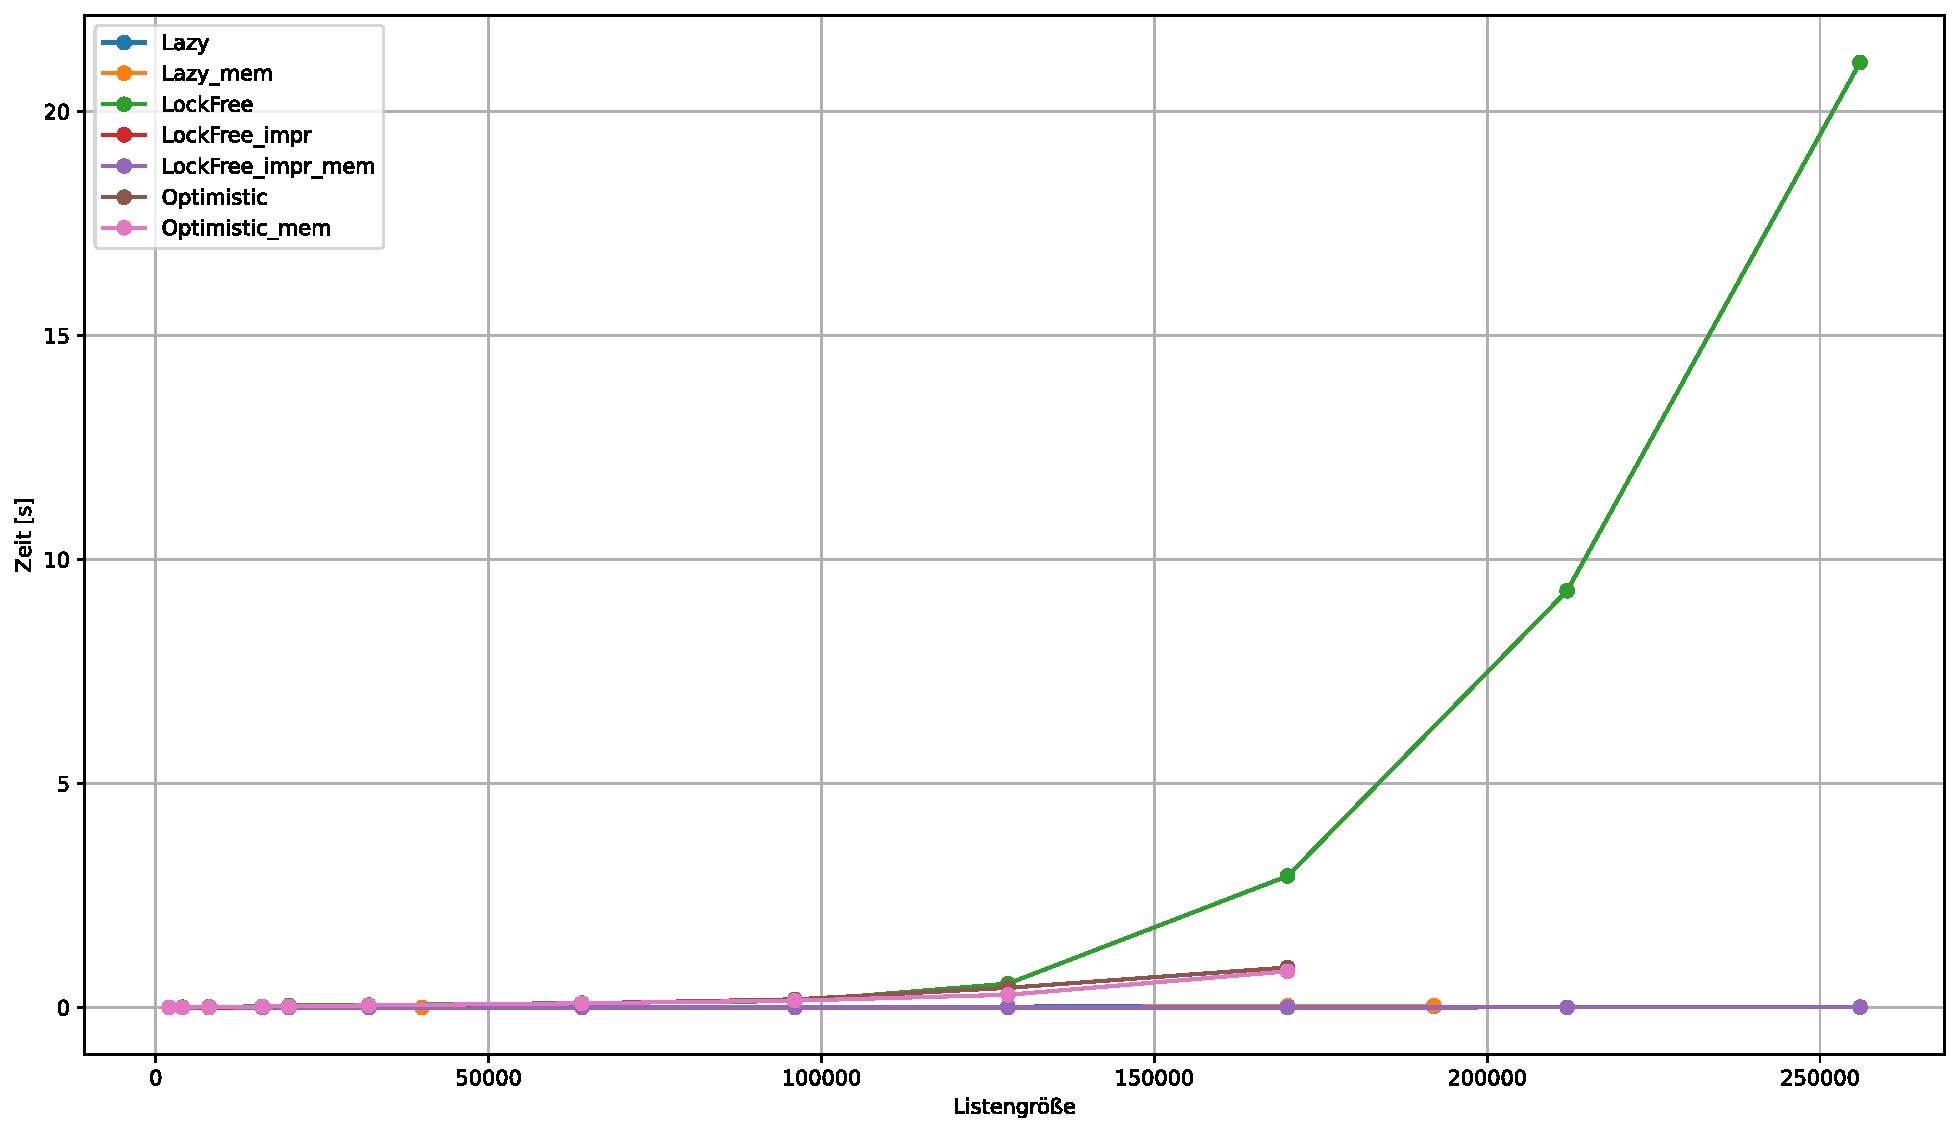
\includegraphics[width=1.0\linewidth]{./plots_pdf/mixed_lostTime.pdf} 
	\caption{Zusätzliche Zeit durch Neustarts}
	\label{fig:mixed_lostTime} 
\end{figure}


%%%%%%%%%%%%%%%%%%%%%%%%%%%%%%%%%%%%
\subsection{Laufzeit mit unterschiedlichen Cores}
\label{subsec:laufzeit}
Die Abbildung \ref{fig:mixed_time_cores_20000} zeigt die Laufzeit mit einer Listengröße von 20000 Einträgen bei
 \textit{contain()}, 1000 \textit{add()} und 100 \textit{remove()} zugriffen.
 Auffallend ist hier, dass
 das \textit{fine-grained locks} mit zwei Cores fast drei mal so lange benötigt als mit einem Core, da sich die einzelnen
 Threads gegenseitig behindern. 
 \todo[]{Warum??}
 Weiters ist auch ersichtlich, dass bei der \textit{coarse-grained locks} Liste die Laufzeit erhöht wird, je höher
 die Anzahl der verwendeten Cores.\\
 Vergleicht man die jeweils schnellsten Datenstrukturen, kommt man auf folgende Ergebnisse:
 Ein Core mit der \textit{coarse-grained locks} Liste benötigt 4636 Sekunden und 64 Cores mit der \textit{lock-free improved with memorymanagement} Liste benötigen 311 Sekunden.
 Das entspricht einen Speedup von 14,9. \\
 Vergleicht man nun den Speedup der jeweils Schnellsten Datenstrukturen bei 20000 Listeneinträgen zwischen einem und zwei Cores mit den Speedup von 32 und 64 Cores, 
 dann erhält man folgende Ergebnisse:
 \\Seedup T1/T2=1,3 
 \\Seedup T2/T4=1,94 
 \\Seedup T8/T16=1,64 
 \\Seedup T16/T32=1,31
 \\Seedup T32/T64=1,43

 \begin{figure}[H]
	\centering
	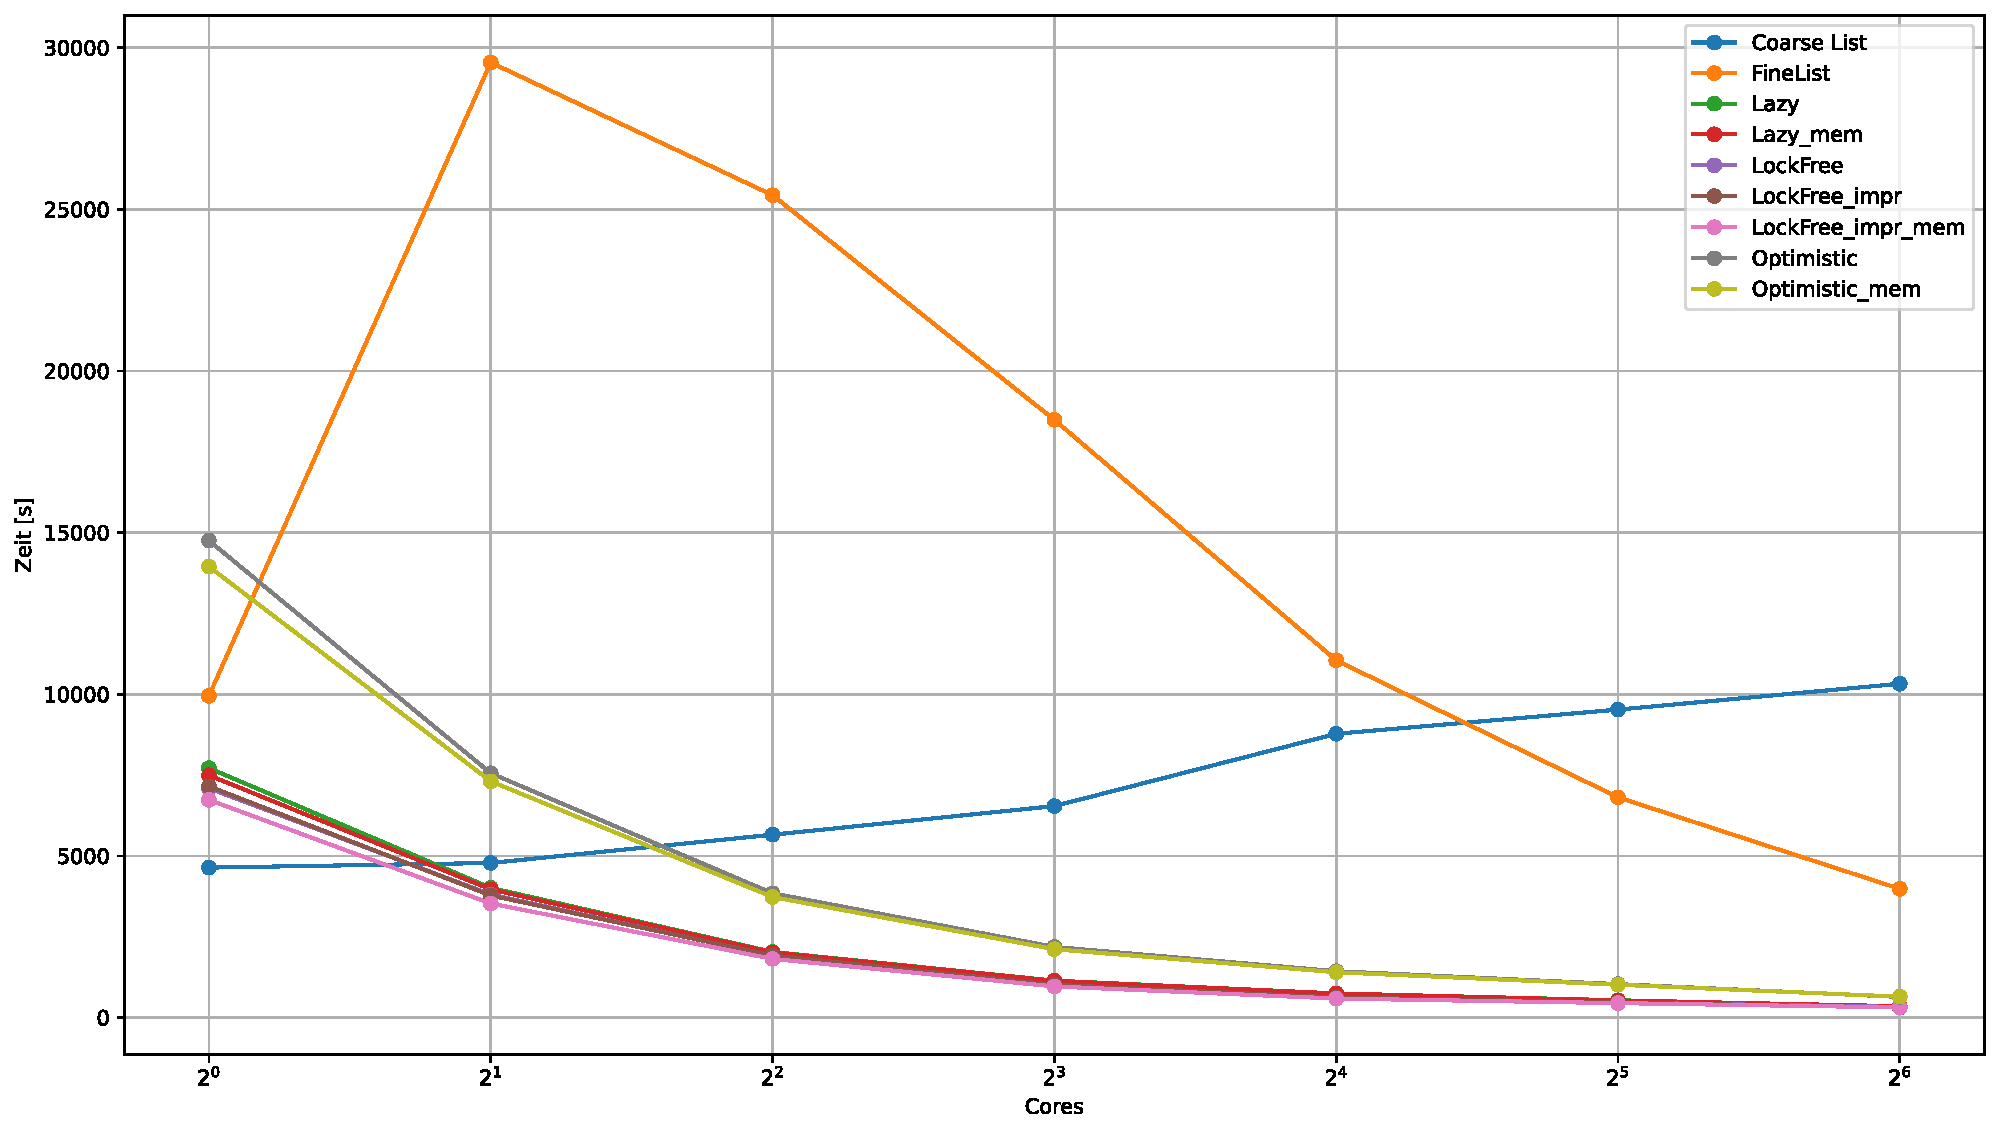
\includegraphics[width=1.0\linewidth]{./plots_pdf/mixed_time_cores_20000.pdf} 
	\caption{Laufzeit mit 20 000 Listeneinträgen} 
	\label{fig:mixed_time_cores_20000} 
\end{figure}

 \subsubsection{Vergleich 40 000 Listeneinträgen}
 \label{subsub:Vergleich_40000}
 Um die schnelleren Datenstrukturen besser zu vergleichen zu können, zeigt Abbildung \ref{fig:mixed_time_cores_40000} die Laufzeit mit verschiedenen Cores
mit der doppelten Anzahl an Listeneinträgen und zugegriffen. 
Vergleicht man nun die Speedups der schnellsten Datenstruktur (\textit{lock-free improved with memorymanagement})
mit 40 000 Einträgen, kommt man auf folgende Werte:
\\Seedup T16/T32=1,37
\\Seedup T32/T64=1,65


\begin{figure}[H]
	\centering
	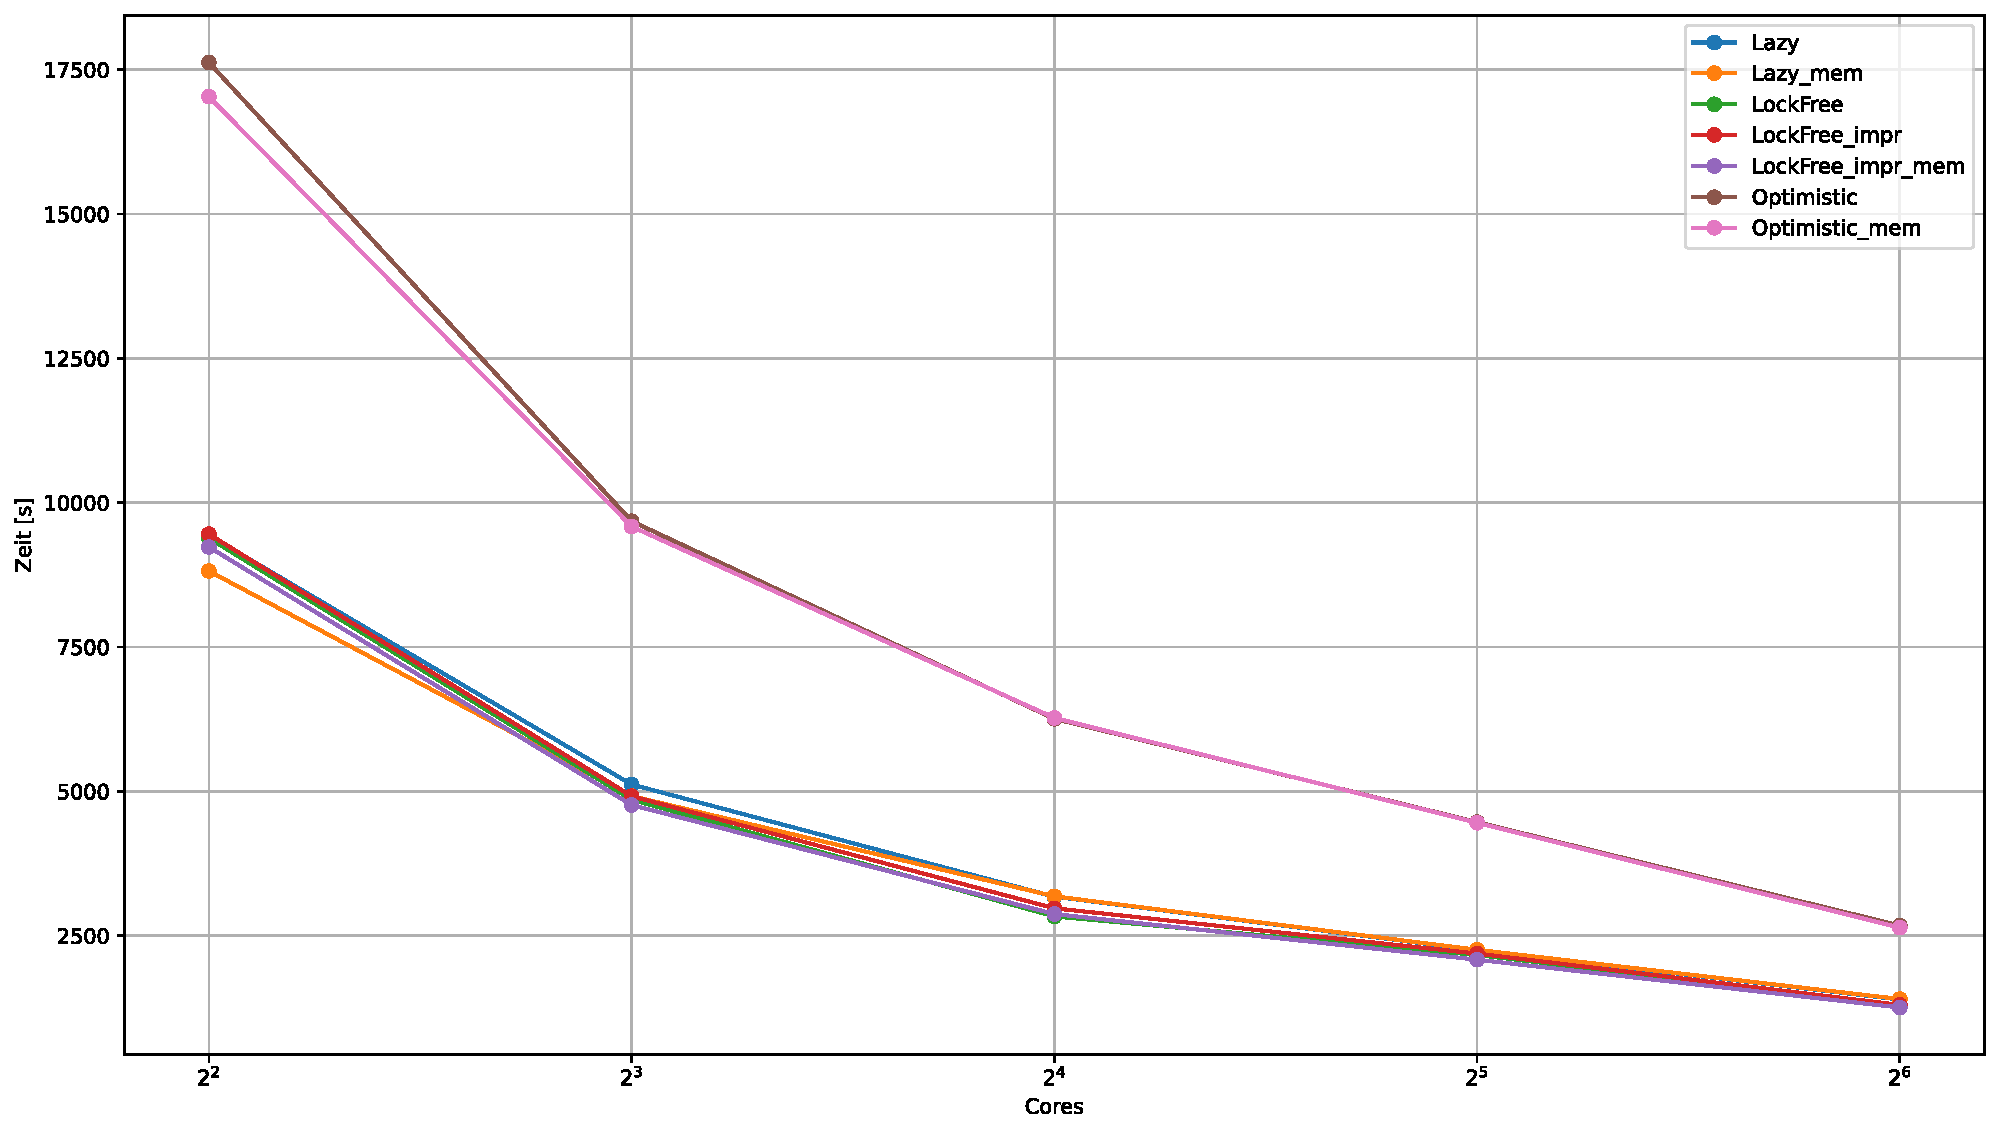
\includegraphics[width=1.0\linewidth]{./plots_pdf/mixed_time_cores_40000.pdf} 
	\caption{Laufzeit mit 40 000 Listeneinträgen}
	\label{fig:mixed_time_cores_40000} 
\end{figure}

\subsubsection{Vergleich 120 000 Listeneinträgen}
Die Abbildung \ref{fig:mixed_time_cores_120000} zeigt die Laufzeit bei
120 000 Listeneinträgen mit 240 000 zugriffen mit der gleichen Aufteilung wie die beiden vorangegengenen Abbildungen.
Vergleicht man nun die Speedups der schnellsten Datenstruktur (\textit{lock-free improved with memorymanagement} Liste)
mit 120000 Einträgen, kommt man auf folgende Werte:
\\Seedup T16/T32=1.42
\\Seedup T32/T64=1,7
\\ Vergleicht man diese Werte mit den Speedups von \ref{subsec:laufzeit} und \ref{subsub:Vergleich_40000}, 
ist ersichtlich, dass das vergrößern der Liste keinen signifikanten Einfluss auf den Speedup hat. 



\begin{figure}[ht!]
	\centering
	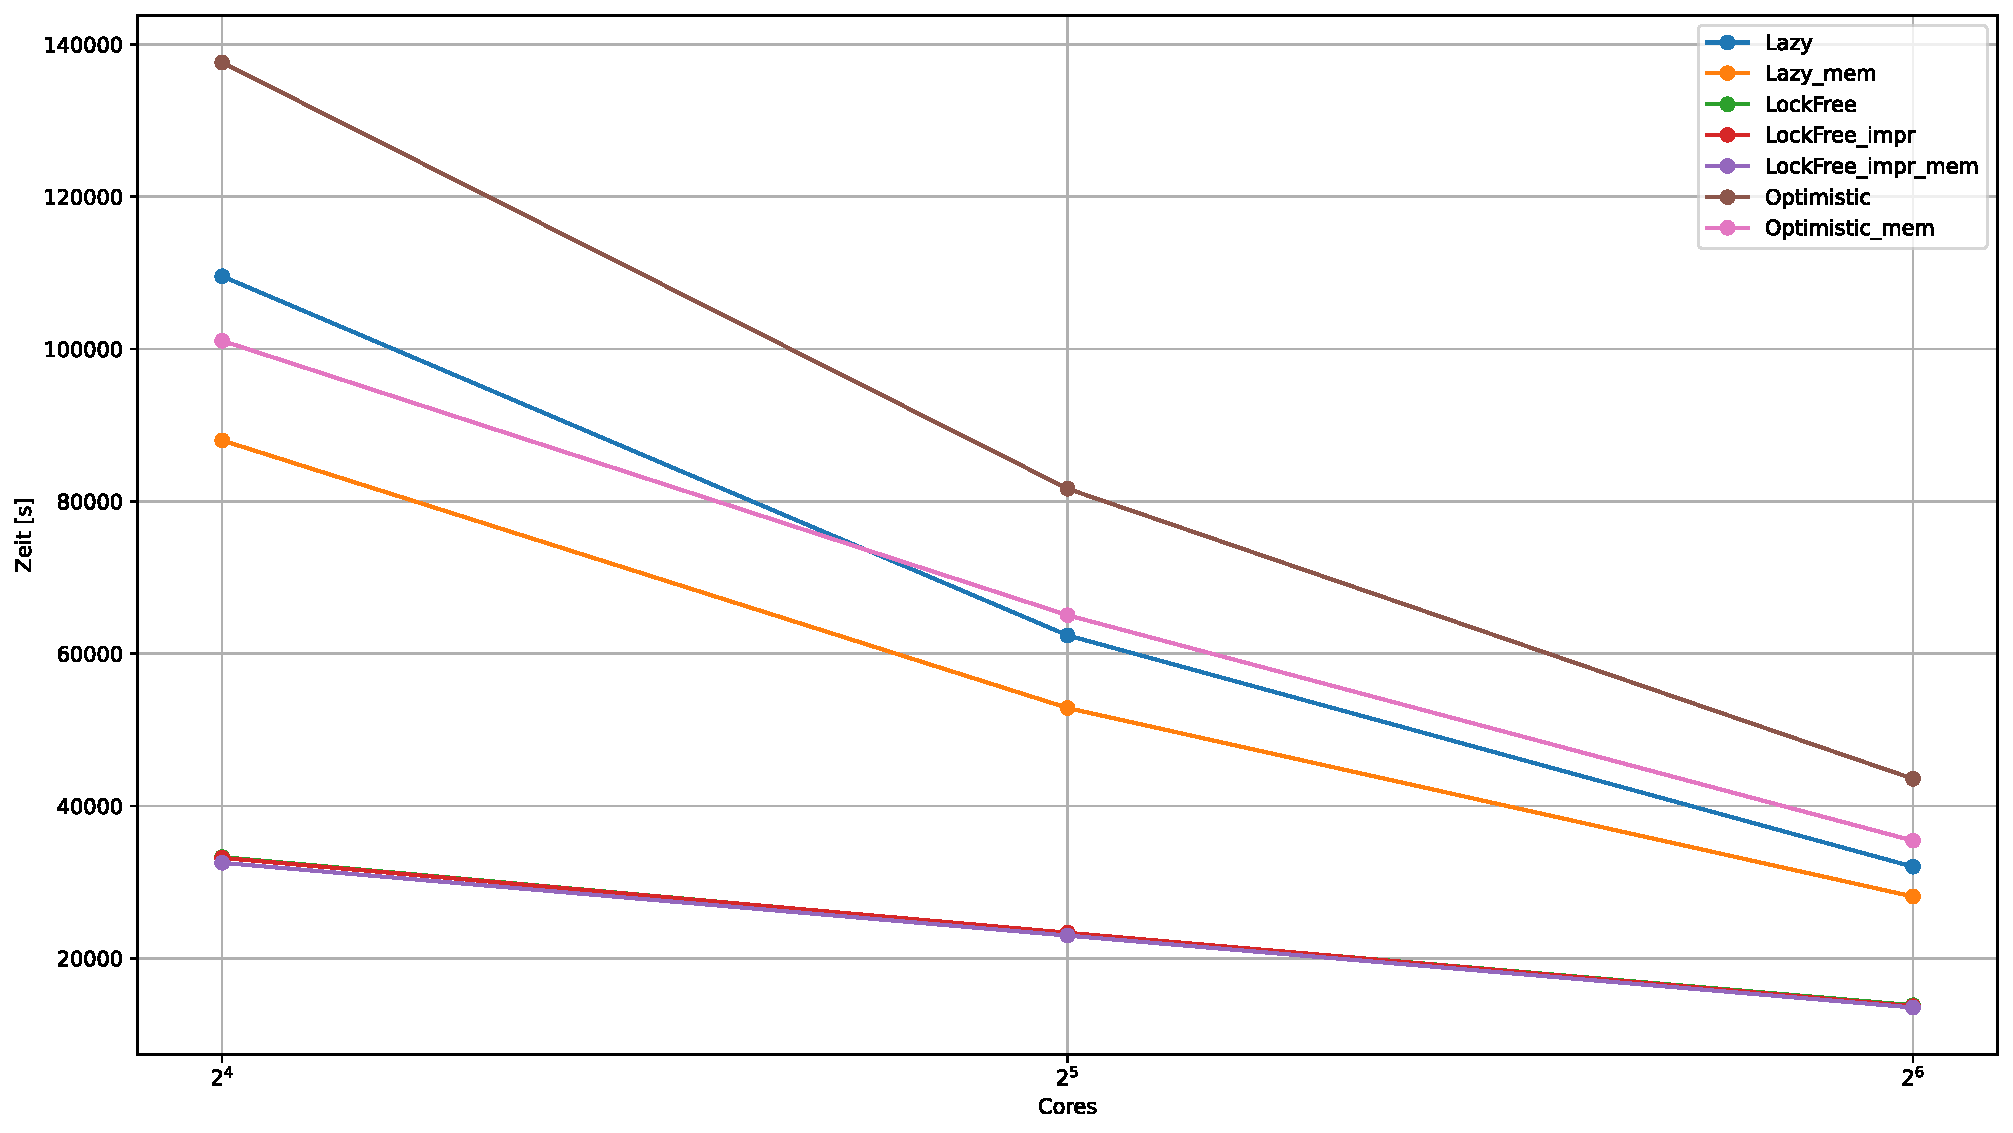
\includegraphics[width=1.0\linewidth]{./plots_pdf/mixed_time_cores_120000.pdf} 
	\caption{Laufzeit mit 120 000 Listeneinträgen}
	\label{fig:mixed_time_cores_120000} 
\end{figure} 
\section{Fazit}
Es wurden Unterschiedliche List-baset Sets implementiert und die Performance evaluiert.
Hierbei wurde zwei Kategorien untersucht. Zum einen die Performance bei steigender Listengröße und
die Laufzeit mit unterschiedlicher Anzahl von Cores. 
Es war ersichtlich, dass bei der Verendung von nur einen Core die Liste mit 
einem globalen Lock am schnellsten ist. Schon ab der Verwendung von 2 Threads sind
andere Listen besser. Es hat sich auch gezeigt, dass das Memmorymanagment, also das zurückgeben
von nicht mehr verwendeten Speicher, positive auswirkungen auf die Performance. Ein weiteres
interessantes Resultat war, dass sich die Laufzeit bei der Liste mit \textit{fine-grained locks} mit zwei Threads 
im Vergleich zu einem Thread fast verdreifacht. Es war auch gezeigt, dass Listen bei einer Kollision
mit anderen Threads abbrechen müssen und dadurch wieder beim Listenkopf beginnen müssen. 
Dieses Verhalten kann mit geringen Programmieraufwand erheblich verbessert werden. Hierbei 
gibt es jedoch noch weiteres Verbesserungspotential. \\
Ein weiteres nicht erwartetes Ergebnis war, dass die \textit{lazy} Liste für eine \textit{contain()} Abfrage
erheblich länger benötigt als die \textit{lock-free} benötigt, obwohl die Funktionen fast identisch sind. 
In diesen Projekt sind alle Zugriffe in zufälliger Reihenfolge erfolgt. Eine weitere Möglichkeit, die Performance
zu evaluieren, wäre der Zugriffen welche nicht gleichverteilt sind. Da die Dichte der Zugriffe auf einigen
Stellen der Liste dadurch höher wird, ist davon auszugehen, dass sich die Performance dadurch verändert. 
Dies wurde hier jedoch nicht behandelt und wäre eine Möglichkeit für ein zukünftiges Projekt. 



		

\end{document}
